\chapter{Circuit Compression} \label{chap:compression}
As discussed in Section \ref{sec:multi_qubit_gates}, the workhorse resource for quantum computing is entanglement.
Unfortunately, entanglement also contributes to the fragility of qubits. Entangled qubits in current noisy intermediate-scale quantum (NISQ) devices \cite{Preskill_2018} are extremely sensitive to environmental interactions, causing rapid quantum decoherence \cite{SCHLOSSHAUER20191}, which leads to the degradation of the entangled state \cite{PhysRevLett.93.140404}.
Another problem of NISQ devices is error propagation. Even with little noise, single-qubit errors spreading throughout the quantum circuit can negate any quantum advantage \cite{PRXQuantum.3.040326}. One way to combat these errors are quantum error correction (QEC) algorithms, which can determine whether an error has occured by a suitable measurement and then applying Unitary corrections \cite{QuantumErrorCorrection}. This chapter however investigates another way of mitigating errors -- quantum circuit compression -- by utilizing higher dimensional systems known as \emph{qudits}. By reducing the number of quantum information carriers, the performance of experimental setups can be improved, while simultaneously lowering the resource requirements for quantum error correction through a reduction in entangling-gate count \cite{gao2023role}.
\section{Qudits}
  As discussed in section \ref{sec:particle_in_a_box}, physical systems are not only limited to two states, in fact, most degrees of freedom of physical systems naturally posess more than two eigenstates.
  As qubits are modeled as two-state systems, they lack the capability to utilize higher dimensions, creating the need for a generalization -- the quantum dit (qudit).
  It represents quantum information in a $d$-dimensional Hilbertspace $\mathcal{H}_d$, where $d>2$. For example, a $4$-dimensional qudit (ququart) can be described using a $4$-dimensional hilberstspace $\mathcal{H}_4$ with the computational basis states $\{\ket{0},\ket{1},\ket{2},\ket{3}\}$.
  Such a quqart can be modeled by a composite system of two qubits by encoding the basis states of the quqart onto the composite systems product states $\{\ket{00},\ket{01},\ket{10},\ket{11}\}$ living also on a $4$-dimensional Hilbertspace $\mathcal{H}_4=\mathcal{H}_2\otimes\mathcal{H}_2$. The key difference is, that gates that are capable to entangle qubits, like $CX$ or $CZ$ gates, act locally rather than entangling when applied to a single ququart state:
  \begin{equation}
    \label{eq:quqart_cx_local_gate}
    \begin{split}
      CX\ket{0}&=\ket{0} \\
      CX\ket{1}&=\ket{1} \\
      CX\ket{2}&=\ket{3} \\
      CX\ket{3}&=\ket{2}.
    \end{split}
  \end{equation}
  So by combining qubits to qudits, the amount of entangling operations in a circuit can be reduced, with the limitation being the existence of a real physical system that can accurately represent the qudit.
  \subsection{Qudit Gates}
    When combining $N$ qubits to one qudit it is also critical to understand how arbitrary local qubit gates $U_i$ (\ref{eq:local_qubit_gate_to_qudit_gate}) and entangling qubit gates $U_{i,j}$ (\ref{eq:entangling_qubit_gate_to_qudit_gate}) transform to local qudit gates $U_d$, where $q_i$ and $q_j$ denote qubits being combined, while $i,j \in \{0,1,...,N-1\}$ and $i<j$ and $\mathbbm{1}$ represents the two dimensional identity matrix.

    \begin{equation}
      \label{eq:local_qubit_gate_to_qudit_gate}
      U_d=\mathbbm{1}^{\otimes i}\otimes U_i\otimes\mathbbm{1}^{\otimes N-1-i}
    \end{equation}
    If the entangling qubit gate $U_{i,j}$ acts on qubits which are not adjacent, a transposition matrix $P$ is needed to rearrange the qubits into adjacent positions, as discussed in section \ref{sec:circuit_calculation}, i.e.
    \begin{equation}
      \label{eq:entangling_qubit_gate_to_qudit_gate}
      U_d=P^{-1}_{i+1\mapsto j}\left(\mathbbm{1}^{\otimes i}\otimes U_{i, i+1}\otimes \mathbbm{1}^{\otimes N-2-i}\right)P_{i+1\mapsto j}
    \end{equation}
    To give a better intuition on how qubit-gates transform when merging qubits, it will be demonstrated in the following example.
    \begin{figure}[H]
      \centering
      \includegraphics[width=.7\linewidth]{figures/qubit_circuit.pdf}
      \caption{Qubit circuit with four $H$-gates and three $CZ$-gates. This graphic was created using qiskit \cite{qiskit2024}. The source code can be found in Listing \ref{lst:compression_qubit_circuit_source}.}
      \label{fig:compression_qubit_circuit}
    \end{figure}
    In this example, using the circuit from Figure \ref{fig:compression_qubit_circuit}, the qubits $q_0$ and $q_1$ will be merged into a ququart ${q^4}_0$ and the qubits $q_2$ and $q_3$ will be merged into one ququart ${q^4}_1$. There are two ways how to transform local gates. Either they are transformed each into two local $4$-dimensional ququart gates, that act only on a specific level of the ququart, or all gates of one column are combined to one $4$-dimensional ququart gate. In this example, the latter is used. Two $H$-gates transform into a $H_4$-gate:
    \begin{equation}
      \label{eq:4_dimensional_hadamard}
      H_4=H\otimes H=
      \begin{pmatrix}
        1 &  1 &  1 &  1\\
        1 & -1 &  1 & -1\\
        1 &  1 & -1 & -1\\
        1 & -1 & -1 &  1
      \end{pmatrix}
    \end{equation}
    Two of the $CZ$-gates, that are entangling in the qubit circuit become local in the ququart circuit. Their matrix representation does not change. The last $CZ$-gate will still be entangling in the ququart circuit, so it will transform into a $16$-dimensional ququart gate called $CZ_{16}$, its matrix form must be calculated using equation (\ref{eq:entangling_qubit_gate_to_qudit_gate}):
    \begin{equation}
      \label{eq:8_dimensional_cz}
      CZ_{16}=\mathbbm{1}\otimes CZ \otimes\mathbbm{1},
    \end{equation}
    where $\mathbbm{1}$ denote $2$-dimensional identity matrices. The resulting ququarts have four eigenstates, so at least two classical bits are needed to store the measurement results. The resulting ququart circuit is depicted in Figure \ref{fig:compressed_ququart_circuit}.

    \begin{figure}[H]
      \centering
      \includegraphics[width=\linewidth]{figures/compressed.pdf}
      \caption{Ququart circuit with two $4$-dimensional $H$-gates denoted by $H_4$, two local $CZ$-gates and one $16$-dimensional entangling $CZ$-gate denoted by $CZ_{16}$. The vertically arranged numbers in the $CZ_{16}$-gate show the numbers of the ququarts it acts on. The horizontally arranged numbers show the internal level of the ququart it acts on. It acts on level $1$ of ququart ${q^4}_0$ (which originated from qubit $q_1$) and on level $0$ of ququart ${q^4}_1$ (from original qubit $q_2$). This graphic was created using qiskit \cite{qiskit2024}. The source code can be found in Listing \ref{lst:compression_ququart_circuit_source}.}
      \label{fig:compressed_ququart_circuit}
    \end{figure}
\section{Algorithm}
  One way to decide what qubits to merge is to create a weighted graph from the circuit and then to cluster nodes of that graph based on their edge-weight with their neighbours \cite{gao2023role}. Using the universal gate set $\{U(\phi,\theta,\lambda), CZ\}$ discussed at the end of section \ref{sec:universal_gateset}, the graph is constructed as follows:
  \begin{enumerate}
    \item From every qubit in the circuit create two graph nodes. The first node represents the state $\ket{0}$ while the second node represents the state $\ket{1}$.
    \item For every local gate $U$ add a graph edge with weight $w_l$ connecting the two nodes that originated from the qubit the gate acts on.
    \item For every entangling gate $CZ$ add a graph edge with weight $w_e$ connecting the second nodes of both qubits it acts on.
  \end{enumerate}
  The $CZ$ gate only affects the $\ket{11}$ state, hence edges are only added to the nodes representing a $\ket{1}$ state. This is also the reason why this algorithm only works for this specific gate set. This simplifies the algorithm, however, it makes it important that $w_l>w_e$ is chosen, otherwise the clustering algorithm may attempt to generate qubits with local $CZ$ gates, which is not possible. A visualization of a graph created from the circuit from Figure \ref{fig:compression_qubit_circuit} is shown in Figure \ref{fig:graph_from_qubit_circuit}.
  \begin{figure}[H]
    \centering
    \includegraphics*[width=.25\textwidth]{figures/graphs/evolution-0/graph_w.pdf}
    \caption{A graph generated from the example circuit from Figure \ref{fig:compression_qubit_circuit} using the algorithm described above with $w_l=4w_e$. The thickness of the edges represent the weights. Nodes connected with a thick line originated from the same qubit, the $H$-gate binds them together. Nodes connected with a thin line are connected through a $CZ$ gate. This graph was visualized using scikit-network \cite{JMLR:v21:20-412}.}
    \label{fig:graph_from_qubit_circuit}
  \end{figure}
  In the next step a graph clustering algorithm groups highly connected nodes together by giving each node a label. In this implementation, any clustering method can be used. The algorithms \textit{Louvain}, \textit{Leiden} and \textit{K-Centers} from scikit-network \cite{JMLR:v21:20-412} are alredy implemented, but other more specialized algorithms, such as for example \textit{gclu} \cite{Sieranoja2021-ik} can easily be added - more on this in section \ref{sec:implementation}.
  \begin{figure}[H]
    \centering
    \scalebox{-1}[1]{\includegraphics*[width=.25\textwidth]{figures/graphs/evolution-0/graph_wl.pdf}}
    \caption{The graph from Figure \ref{fig:graph_from_qubit_circuit} got labeled by the \textit{Louvain} clustering algorithm. Each color represents one label. This graph was visualized using scikit-network \cite{JMLR:v21:20-412}.}
    \label{fig:graph_from_qubit_circuit_labeled}
  \end{figure}
  In Figure \ref{fig:graph_from_qubit_circuit_labeled} the result from labeling the graph from Figure \ref{fig:graph_from_qubit_circuit} is visualized. After labeling, all nodes with the same labels get merged into one new node while preserving edge data in a seperate datastructure, leading to a graph where every node now represents a qubit. Such a graph is visualized in Figure \ref{fig:merged_graph}.
  \begin{figure}[H]
    \centering
    \includegraphics*[width=.25\textwidth]{figures/graphs/evolution-1/graph_w.pdf}
    \caption{This graph is the result of merging every node with the same label from the graph in Figure \ref{fig:graph_from_qubit_circuit_labeled}. Every node now represents a qubit. This graph was visualized using scikit-network \cite{JMLR:v21:20-412}.}
    \label{fig:merged_graph}
  \end{figure}
  This step did not produce a graph representing a qudit circuit but a graph representing a qubit circuit. Therefore, the clustering algorithm is applied again on the new graph, resulting in a ququart circuit graph, shown in Figure \ref{fig:ququart_graph}.
  \begin{figure}[H]
    \centering
    \begin{subfigure}{.25\textwidth}
      \centering
      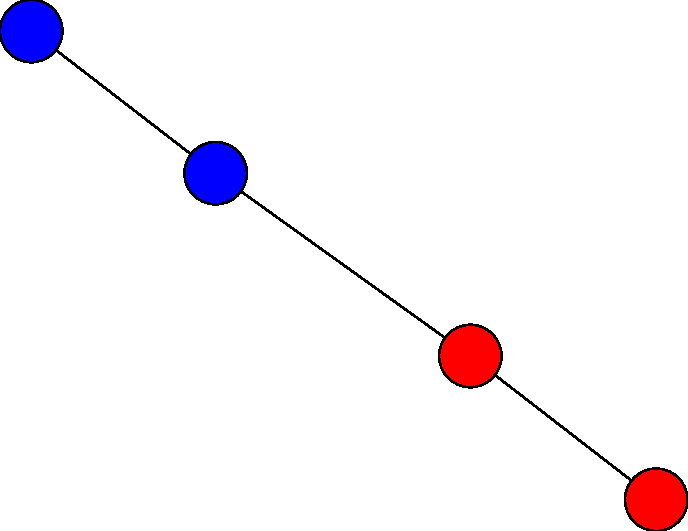
\includegraphics[width=\linewidth]{figures/graphs/evolution-1/graph_wl.pdf}
      \caption{}
    \end{subfigure}%
    \begin{subfigure}{.25\textwidth}
      \centering
      \scalebox{-1}[1]{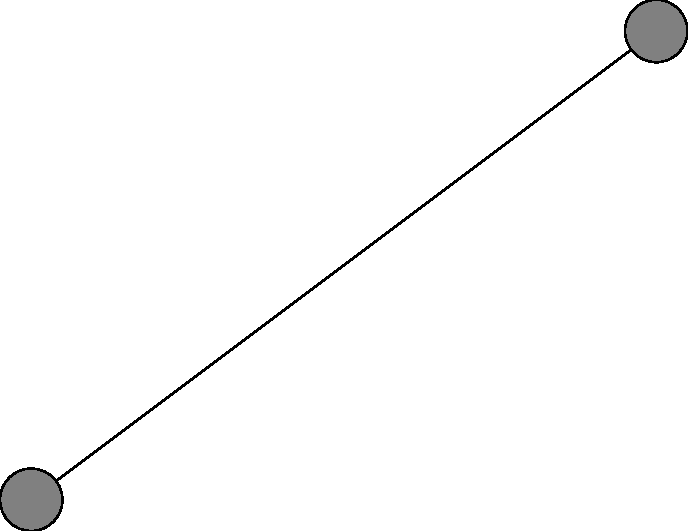
\includegraphics[width=\linewidth]{figures/graphs/evolution-2/graph_w.pdf}}
      \caption{}
    \end{subfigure}
    \caption{The \textit{Louvain} clustering algorithm assigns two labels to the nodes of the graph (a), effectevely merging four qubits into two ququarts. The resulting graph (b) represents exactly the circuit from Figure \ref{fig:compressed_ququart_circuit}. These graphs were visualized using scikit-network \cite{JMLR:v21:20-412}.}
    \label{fig:ququart_graph}
  \end{figure}
  In summary, the algorithm can be described as follows:
  \begin{enumerate}
    \item Create a weighted graph from a circuit
    \item Run a clustering algorithm $c$ that assigns labels to nodes of the graph
    \item Save all gate information from each cluster in a seperate datastructure
    \item Merge all nodes with the same label
    \item Repeat steps 2. to 4. $n$ times
  \end{enumerate}
  where $c$ and $n$ can be chosen depending on the wanted dimension $d$ of the qudit and width of the qubit circuit.
\section{Implementation} \label{sec:implementation}
  The entire source code of the project is publicly available at \url{https://github.com/SimShady/qudit-compression} licensed under the GNU General Public License version 3 \cite{gplv3}. A copy of the source code can also be found in Appendix \ref{sec:project_source}. The project is structured in the following folders and files:
  \begin{itemize}
    \item \texttt{circuits/}
    \begin{itemize}
      \item In this folder, all input circuits are stored in OpenQASM-format \cite{qasm}. Except for the file \texttt{thesis\_circuit\_qiskit\_4.qasm}, every file in this folder is taken from the mqt-qudit-compression project \cite{mato2023compression}.
    \end{itemize}
    \item \texttt{solutions/}
    \begin{itemize}
      \item In this folder, all output circuits and visualizations are stored.
      \item Circuit data is stored in \texttt{solutions/<circuitname>/<algorithmname>/data}
      \item Visuals are stored in \texttt{solutions/<circuitname>/<algorithmname>/visuals}
    \end{itemize}
    \item \texttt{graph.py}
    \item \texttt{circuit.py}
    \item \texttt{clustering.py}
    \item \texttt{processing.py}
    \item \texttt{main.py}
    \item \texttt{circuitinfo.py}
    \item \texttt{requirements.txt}
    \item \texttt{flake.nix}
    \item \texttt{flake.lock}
\end{itemize}
In the following, the source files are described in more detail.
\subsection*{{\Large\texttt{graph.py}} (Listing \ref{lst:graph.py})}
  This file provides a simple datastructure to model a graph using only a list of edges to do so. That means, that if during the clustering process a node loses all edges it is destroyed. That has to be kept in mind when analysing results. Additionaly, an array \texttt{node\_weights} is maintained that keeps track of the size of each node, with the size meaning the number of original nodes it has been merged with. The datastructure has basic methods to create and copy it as well as two special methods \texttt{get\_reduced\_graph\_by\_label} and \texttt{reduce\_graph}.
  \begin{itemize}
    \item \texttt{get\_reduced\_graph\_by\_label} creates a new graph based on provided labels. It is a helper function for \texttt{reduce\_graph}.
    \item \texttt{reduce\_graph} calls the provided clustering algorithm one or more times and creates new graphs while keeping track of the history of graphs and labels used. These history arrays are then returned.
  \end{itemize}
\subsection*{{\Large\texttt{circuit.py}} (Listing \ref{lst:circuit.py})}
  This file contains every datastructure needed to describe a qudit circuit.
  \begin{itemize}
    \item \texttt{Instruction}
    \item \texttt{Qudit}
    \item \texttt{QuditGate}
    \item \texttt{Circuit}
  \end{itemize}
  The \texttt{Instruction} class is just a helper structure that is used to convert qiskit circuits into an instance of \texttt{Circuit}. The classes \texttt{Qudit} and \texttt{QuditGate} are mainly structures to store data about qudits and gates. They have a function to serialize to JSON and some error handling to prevent invalid states. The most important datastructure is the \texttt{Circuit}. It stores a list of qudits and a ordered list of qudit gates, and can be created by passing such two lists to the constructor or from a QASM file. It also has a method to serialize to JSON which calls the serializers of its qudits and gates. The two important methods in this class are:
  \begin{itemize}
    \item \texttt{generate\_weighted\_graph}, which converts the circuit to a weighted graph. The weights $w_l$ and $w_e$ can be chosen. The defaults are $w_l=400$ and $w_e=100$. The implementation of converting a qiskit circuit into a graph was based on the mqt-qudit-compression project \cite{mato2023compression}.
    \item \texttt{get\_updated\_circuit\_by\_labels}, which creates a new circuit based on the current circuit and a set of labels from a graph clustering algorithm.
  \end{itemize}
\subsection*{{\Large\texttt{clustering.py}} (Listing \ref{lst:clustering.py})}
  This file is used as a library for clustering algorithms and also serves as example on how the interface of a clustering function needs to look like to be compatible with this project. A clustering function needs to take a \texttt{Graph} for an argument and return a list of integers representing the labels. The index $i$ of this list denotes the number of the node, while the value at $i$ denotes the label. If additional parameters need to be passed to the underlying clustering function, this can be done using a higher order function demonstrated by the three implemented functions \texttt{louvain}, \texttt{leiden} and \texttt{kcenters}.
\subsection*{{\Large\texttt{processing.py}} (Listing \ref{lst:processing.py}) and {\Large\texttt{main.py}} (Listing \ref{lst:main.py})}
  The file \texttt{processing.py} provides a function that prepares and applies the compression of one circuit using one clustering algorithm. It writes the resulting circuit data and visuals including the history to the \texttt{solutions} folder. The file \texttt{main.py} serves as entrypoint of the program. It looks up all files in the \texttt{circuits} folder and processes each circuit with multiple clustering algorithms using the function from \texttt{processing.py}.
\subsection*{{\Large\texttt{circuitinfo.py}} (Listing \ref{lst:circuitinfo.py})}
  This program serves as utility to inspect generated circuits. For the example circuit from Figure \ref{fig:compressed_ququart_circuit}, it prints: 
  \begin{verbatim}
Number of qudits: 2
Qudit dimensions: [4, 4]
Number of local gates: 6
Number of entangling gates: 1
  \end{verbatim}
  Or for a circuit a little bit more complex (from \texttt{qpeexact\_indep\_qiskit\_31.qasm}):
  \begin{verbatim}
Number of qudits: 7
Qudit dimensions: [38, 4, 4, 4, 4, 4, 4]
Number of local gates: 1408
Number of entangling gates: 571
  \end{verbatim}
\subsection*{Utility files}
  The files \texttt{requirements.txt} (Listing \ref{lst:requirements.txt}), \texttt{flake.nix} (Listing \ref{lst:flake.nix}), \texttt{flake.lock} (Listing \ref{lst:flake.lock}) handle dependency management and support the reproducibility even years after this writing. \texttt{requirements.txt} is used by the python package manager \textit{pip} to install the correct versions of python packages that the project depends on. The other two files are used by Nix \cite{Nix} to create a development shell that replicates the exact environment as it exists at the time of writing. This shell can be activated using the command \texttt{nix-shell}.
